% Document

\IEEEdisplaynontitleabstractindextext
\IEEEpeerreviewmaketitle
\ifCLASSOPTIONcompsoc
\IEEEraisesectionheading{\section{Introduction}\label{sec:introduction}}
\else
\section{Introduction}
\label{sec:introduction}
\fi

\IEEEPARstart{C}{ode} completion, or AutoCompletion, is one of the most essential features in modern \gls{ide} (e.g., GitHub's Copilot, Intellisense in Visual Studio Code \cite{intelliSense}).
% Tabnine\footnote{https://www.tabnine.com}
The goal of code completion is to automatically recommend source code based on a given context, which could help developers reduce the amount of typing and coding iteration time and eliminate the number of typo errors.
A recent study conducted by Google found that the current code completion feature could reduce developers' effort by 6\% and context switching by 7\%~\cite{ml2022google}.

% the next source code statements given the current context. It can help improve developers productivity by minimize the amount of typing and eliminate typos. These may include pop-up when typing, suggest methods or objects, or query parameters of functions.
% \kla{better to mention the existing tools too, e.g., intellisense, tabnine}\
% \kla{also better to mention the benefit https://ai.googleblog.com/2022/07/ml-enhanced-code-completion-improves.html / check this link and put the reference.}
% Some existing tools are, for example, the code completion in IntelliSense \cite{intelliSense} which is a part of code editing features in Visual Studio Code (VS Code), and Tabnine \footnote{https://www.tabnine.com} which is the AI code assistant for whole-line and full-function code completion that can integrate to many \gls{ide} platforms.

% \kla{2nd para should start from recent work, not the history. this para can be in the related work.}

Recent code completion approaches often leverage modern deep learning architectures (e.g., Recurrent Neural Network, Transformer architecture) to exploit their strong representation power.
More specifically, state-of-the-art code completion models (e.g., CodeGPT~\cite{lu2021codexglue}, GPT-2~\cite{radford2019language}, GPT-C~\cite{svyatkovskiy2020intellicode}, TavTrans~\cite{kim2021code}, CodeFill~\cite{izadi2022codefill}) are based on code-focused large language models (LLMs) that are trained from large codebase and natural language corpora (e.g., the CodeSearchNet corpus with 2 million GitHub repositories). These LLMs are fine-tuned on a specific dataset to perform specific tasks (e.g., code completion).
However, existing code completion approaches have the following limitations.

% For example, Li~\ea~\cite{li2017code} proposed a Pointer Mixture Network model that incorporates the AST information.
% Svyatkovskiy~\ea~\cite{svyatkovskiy2019pythia} proposed Pythia, which is a Long Short-Term Memory (LSTM) network ??? with AST.
% Therefore, researchers proposed to leverage a Transformer architecture, addressing the various limitations of the RNN-based architecture~\cite{kim2021code, liu2020self, izadi2022codefill, liu2022unified}.
% However, such RNN-based and LSTM-based models often suffer from long-term dependencies ???? \kla{what are the limitations of RNN so Transformer is proposed}.


% \kla{bra bra bra , how does it incorporate AST information?}.
% \kla{CodeFill?}


% applying multi-task learning with \gls{ast} \cite{liu2020self}  \cite{izadi2022codefill} \cite{liu2022unified} 
% TravTrans / Transformers+AST  
% GPT-2 (Decoder-only Transformer)
% CodeGPT (Pre-trained Decoder-only Transformer)
% CCAG = flattened \gls{ast} as graphs +  GNN \cite{wang2021code}
% Line-level completion (\cite{wang2020towards}  \cite{izadi2022codefill}
% CodeGPT \cite{lu2021codexglue}
% For code completion in research field, recently it is formulated to an \gls{nlp} task \cite{hindle2016naturalness}. 
% Afterward, many modern NLP techniques has been applied to solve code completion task. For instance, the GPT-style model such as GPT-2 \cite{radford2019language} and language modelling objective have been applied to train with code dataset \cite{lu2021codexglue}. However, some work present that the direct code sequences sometime fail to produce the syntactically correct code \cite{brockschmidt2018generative}, therefore the code language grammar such as \gls{ast} are presented to be utilized to learn the syntactical structures. Many recent works have make use of \gls{ast} for code completion. For instance: 
% . These yield the promising results in code completion.
% using \gls{ast} with LSTM \cite{svyatkovskiy2019pythia},


% From 2012, code completion is migrate \kla{not migrate, but better say 'formulated as an NLP task'? not sure if this is your intention} to \gls{nlp} problem by Hindle et al. \cite{hindle2016naturalness}. Afterward, many NLP techniques has been applied to solve code completion task. There are some works present that the direct code sequences sometime fail to produce the syntactically correct code \cite{brockschmidt2018generative}, therefore the code language grammar such as \gls{ast} are presented to be utilized to learn the syntactical structures. Many recent works have make use of \gls{ast} for code completion \cite{wang2021code} \cite{wang2020towards} \cite{svyatkovskiy2019pythia} \cite{kim2021code} \cite{izadi2022codefill} \cite{liu2020self} \cite{liu2022unified} and yield the promising results.
% \kla{this section needs more details what is each technique and how AST is used?}

\textbf{Limitation 1: \emph{On-the-fly code completions approaches do not consider syntactic information.}}
On-the-fly code completion approaches are designed to generate code tokens based on a given context without requiring the completeness of prior context.
Represent techniques include GPT-2~\cite{radford2019language}, a Transformer-based decoder model for generative tasks pre-trained on English webpage datasets; CodeGPT~\cite{lu2021codexglue}, a GPT-2 model architecture pre-trained on source code datasets; and GPT-C~\cite{svyatkovskiy2020intellicode}, a GPT-2 model architecture pre-trained on multi-language source code. In their pre-training, these models learn to complete the next code tokens. 
In doing so, the performance of these on-the-fly code completion approaches is limited by their lack of consideration of syntactic information.
% provided in the source code.

\textbf{Limitation 2: \emph{Existing syntax-aware code completion approaches are not on-the-fly.}}
To ensure that the generated source code is syntactically correct~\cite{brockschmidt2018generative}, researchers proposed to leverage the Abstract Syntax Tree (AST) information~\cite{li2017code, svyatkovskiy2019pythia, kim2021code, liu2020self, izadi2022codefill, liu2022unified}.
For example, Kim~\ea~\cite{kim2021code} proposed TravTrans, 
% \kla{not clear yet, tell what is this approach}
a Transformer-based architecture consuming syntactic information from a variety representations of ASTs traversal;
Izadi~\ea~\cite{izadi2022codefill} proposed CodeFill, a multi-task,  
% \kla{parallel is a new jargon that is never clearly defined. avoid using it.}
Transformer-based architecture consuming source code and AST types. 
While existing AST-based code completion approaches may generate code that is more syntactically correct, the application scenario remains limited.
In particular, the existing AST-based code completion approaches~\cite{li2017code, svyatkovskiy2019pythia, kim2021code, liu2020self, izadi2022codefill, liu2022unified} require source code to be completed (i.e., all the previous tokens are valid and parsable) at the inference time so the AST information can be obtained from the source code.
However, our motivating analysis found that in practice, two thirds of the source code characters is incomplete and not parsable (e.g., containing syntax errors), making the existing AST-based code completion approaches \emph{inapplicable} in real-world scenarios.
% Second, existing AST-based code completion approaches~\cite{li2017code, kim2021code, izadi2022codefill} are designed to predict an individual code token at the AST node level, not the natural sequence of source code.
% \kla{will mention this later.}



% still focus on the AST node prediction task (i.e., predicting the next AST node based on a given sequence).
% However, such prediction generate the token individually and could not generate the whole line in practical.
% For instance, in Fig.~\ref{fig:motivation} an equivalent source code of an AST node is \textit{logging.getLogger()}, but if we generate the AST node, the \textit{dot} and \textit{parenthesis} characters are not generated. \kla{may be adding an illustrative example figure here. - make a case about on-the-fly....}
% Thus, the AST node prediction can generate only some tokens and not the whole line. 



% However, in real-world scenario, \gls{ast} information is difficult \kla{difficult does not mean possible or impossible} to be correctly retrieve because the syntactically correct and complete source code is hardly present in code completion problems \cite{svyatkovskiy2020intellicode}. \kla{better say what is required to obtain AST information. but in the real-world it may not be available} \kla{it would be great to give an example? ... } Therefore, we propose the use of standard token type information instead of \gls{ast}. The standard token type information can also learn the syntactical data similar to \gls{ast} and more simple to use. It does not require the completeness for parsing and can be retrieve at any points of source code. We present in this work that this information could be useful for code completion.


% However, the evaluation of these papers does not focus on the primary objective of the code completion tasks (i.e., predicting the next code token based on a given sequence of source code).

% However, in real-world scenarios, there are some drawbacks using AST in code completion. Firstly, prediction on \gls{ast} node sequences is not reflect the actual performance of code completion, as it is not the natural order of typing \cite{liu2020multi}. Secondly, AST could create additional overhead and dependencies \cite{svyatkovskiy2020intellicode}. More importantly, last but not least, the syntactically correct and complete source code is hardly present in code completion problems, therefore the ASTs information which required the parse-able code tend to be not available in practical. 

% From the example in Fig. \ref{fig:ASTvsType} and Fig. \ref{fig:ASTfailvsType}. We can observe that the code in Fig. \ref{fig:ASTvsType}a still be able to parse to AST as a result in Fig. \ref{fig:ASTvsType}b. However, with one additional '=' sign in code in Fig. \ref{fig:ASTfailvsType}a, it raises error in AST result in Fig. \ref{fig:ASTfailvsType}b.


\emph{In this paper}, we propose \our, an automated code completion approach that can generate source code at any time regardless of the completeness of the source code, i.e., \textbf{syntax-aware on-the-fly code completion}.
Our approach is designed to consider the syntactic information of the source code during the learning phase, but \emph{does not} require syntactic information during the inference phase.
Instead of using the AST information like in previous works~\cite{kim2021code, izadi2022codefill, li2017code, svyatkovskiy2019pythia, liu2020self, liu2022unified}, we propose to leverage the \emph{token type} information (e.g., String, Number, Name, Keyword), which is a readily-available and light-weight syntactic information without requiring the completeness of the source code.
During the learning process, we design our approach to carry out two prediction tasks, i.e., the token prediction task and the type prediction task.
% Unlike some previous work that leverages AST information as an individual learning objective for the AST node prediction task~\cite{kim2021code,li2017code},
% Our research study on how to best use this token type information along with source code.
To ensure that our model captures both syntactic and semantic information during the training process, we leverage Multi-Task Training (MTT) techniques to learn both the token prediction task and the type prediction task. 
% prediction tasks, and intermediate fine-tuning (STILTs) that sequentially learns from task-to-task.
% To address this challenge of training on multiple tasks (i.e., code prediction and type prediction tasks),
% Particularly, 
Given a sequence of code tokens, our approach performs the following steps: (1) extract the token type information of each token, (2) perform the sub-word tokenization on each token, (3) align token type data with sub-word source code data, and (4) build a code completion model using a GPT-2 architecture based on a pre-trained CodeGPT language model with a multi-task training technique.
% \kla{highlight we don't use the type information at the inference time.}

In our experiment, we compare our \our~with four existing state-of-the-art models (i.e., Pointer Mixture Network~\cite{li2017code}, TravTrans~\cite{kim2021code}, GPT-2~\cite{radford2019language}, and CodeGPT~\cite{lu2021codexglue}).
% \kla{can you add a reference?}).
During the inference phase, we evaluate our approach based on the token-level and line-level prediction tasks.
Through an extensive evaluation on the \textit{PY150}~\cite{raychev2016probabilistic} standard benchmark Python dataset for the code completion task that is used in Microsoft's CodeXGLUE benchmark~\cite{lu2021codexglue}, we answer the following research questions:

% \kla{revised till here}

\begin{description}[leftmargin=1cm, itemsep=3pt]
  \item[RQ1)] \textbf{\rqone}\\
  \textbf{Results.} \fdone

% \our~achieves the first rank on the CodeXGLUE leaderboard with an accuracy of 77.12\% for the token-level predictions, which is 0.43\%-24.25\% more accurate than other baselines.
% In addition, \our~achieves an exact match of 43.37\% for the line-level predictions, which is 3.63\%-84.73\% more accurate than other baselines.

%   Compared with second-best models, \our~achieves an improvement on accuracy of 1.89\% (from 75.69\% to 77.12\%) in token-level prediction and on exact match of 8.34\% %3.34\% 
%   \kla{use relative percentage} 
%   (from 40.03\% to 43.37\%) in line-level prediction.
  
  \item[RQ2)] \textbf{\rqtwo}\\
  \textbf{Results.} \fdtwo

%   the different training techniques can vary accuracy by 2.98\% %2.23\% (from 74.77\% to 77.00\%) in token-level prediction, and 
%   the exact match is different by 11.86\% (i.e., max-min) %4.54\% (from 38.29\% to 42.83\%) in line-level prediction.
  
  \item[RQ3)] \textbf{\rqthree}\\
  \textbf{Results.} \fdthree
%   When adjusting the weights (section~\ref{sec:approach-weight}) of the two tasks (token type prediction and token value prediction), accuracy in token-level prediction can differ by 2.21\% %1.67\% 
%   (from 75.45\% to 77.1\%) and exact match in line-level prediction can differ by 9.05\% %3.6\%
%   (from 39.77\% to 43.37\%).
%   The results show that \our~can perform better in both token-level and line-level predictions when tuning the task weighing parameters.
  
  \item[RQ4)] \textbf{\rqfour}\\
  \textbf{Results.} \fdfour
%   The different decoding methods can vary the results in line-level prediction by 22.84\% %7.72\% 
%   (from 33.80\% to 41.52\%) on exact match and 7.65\% %5.26\%
%   (from 68.72\% to 73.98\%) on edit similarity.
%   Thus, decoding methods have a significant impact on the quality of predictions, and sampling-based methods may not be suitable for the code completion task.
%   Our best suggestion for decoding method as in our setting is Beam search with beam size of 5.
\end{description}


% Therefore inspired by AST, we propose to use standard tokenizer type information. We run the models for python language. The tokens in python are for examples parenthesis, strings, operators, keywords, and variable names. The reasons we use standard tokenizer type information are because: firstly, it maintains the syntactical information similar to \gls{ast}. Second, it is able to retrieve at any points with minimum false representations. Lastly, it is easy to use along the raw source code because it is generated in the similar natural order of typing sequences. The examples compare between AST parser results and standard type results are shown in Fig. \ref{fig:ASTvsType} and Fig. \ref{fig:ASTfailvsType}. We can see that the standard tokenizer type can be retrieved from both source code resulting in Fig. \ref{fig:ASTvsType}c and Fig. \ref{fig:ASTfailvsType}c. Thus, we have this type prediction as the additional non-target task i.e. auxiliary task.

% There are multiple techniques in order to learn the auxiliary task with target task. Nonetheless, in NLP, two essential techniques \cite{weller2022use} are \gls{mtl} and \gls{ifn} \cite{phang2018sentence}. We leverage these techniques and propose TypeComp - the generative type-aware transformers for code completion in this paper. \kla{better highlight what is the challenge of the existing learning technique so multi-task learning is needed}. We intensively train and test models with different training techniques, weighing, and decoding methods in order to find the best architecture of type-aware model for code completion task. Our work is not limit only to a token-level prediction but also include a line-level prediction. We compete TypeComp to 4 state-of-the-arts, additionally we send the results to evaluate on CodeXGLUE Benchmark for code completion task. The results show that TypeComp surpass all state-of-the-art baselines.  



\textbf{Novelty.} The key novelty of our work is as follows:
% \kla{Wannita updates this part too.}
% \kla{TODO later}
\begin{itemize}
    \item \our~is the first to leverage the token type information for code completion with a variety of multi-task training techniques.
    \item \our~is the first to extensively explore the sensitivity of the task weighting parameter and decoding methods in code completion.
    % \item \our~is the first for an empirical study on decoding methods for code completion
    \item \our~surpasses four state-of-the-art code completion techniques and the CodeXGLUE Benchmark, achieving the highest performance in both token-level and line-level predictions.
    \item \our~is publicly available on HuggingFace (\url{https://huggingface.co/Wannita/PyCoder}) together with the token type dataset (\url{https://huggingface.co/datasets/Wannita/PyCoder}).
\end{itemize}

\textbf{Paper Organization.} 
The paper is organized as follows.
Section~\ref{sec:background} describes the background, motivation, and limitations of the state-of-the-art approaches.
Section~\ref{sec:approach} presents our \our~approach. 
Section~\ref{sec:experiment} describes the experimental setup and state-of-the-art baselines. 
Section~\ref{sec:results} presents the experimental results and discussions. 
Section~\ref{sec:discussion} discusses the results of our \our. 
% Section~\ref{sec:relatedwork} presents the related work.
Section~\ref{sec:threats to validity} discloses the threats to validity.
Section~\ref{sec:conclusion} draws the conclusion. 


% The model architectures on \gls{mtl} and \gls{ifn} are explained in session 3. The experimental part is in session 4 which includes dataset (4.1), model training (4.2), post-processing methods (4.3), and baselines information (4.4). The experimental results from 4 research questions are in session 5. Lastly is the discussion and related works in session 6 and 7.

% \begin{figure}
%     \centering
%     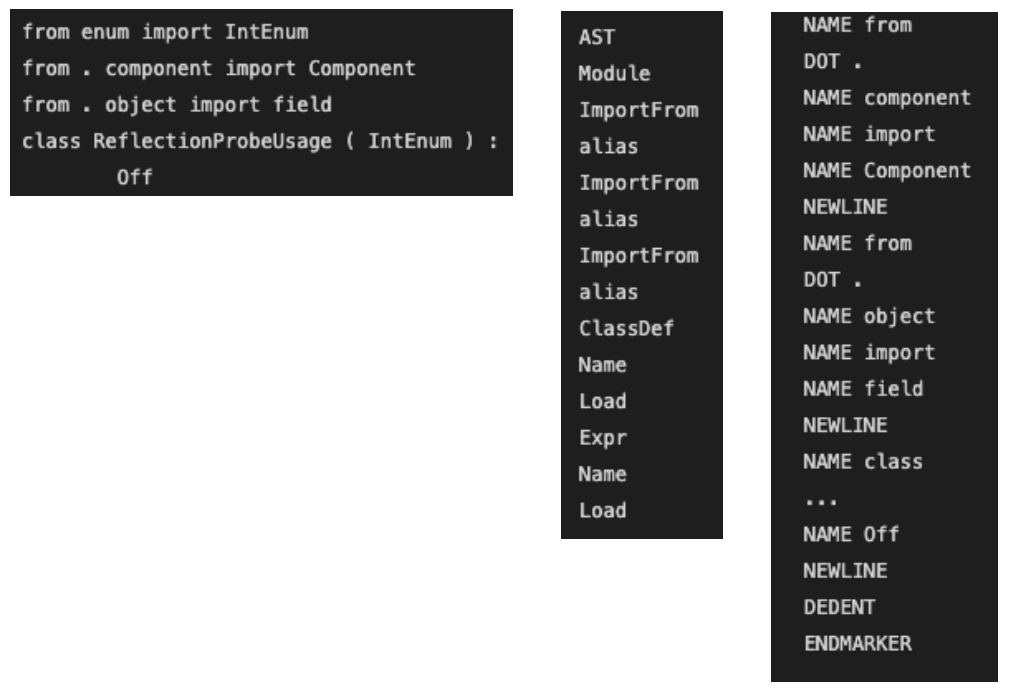
\includegraphics[width=\columnwidth]{figures/motivation2.png}
%     \caption{a) source code example for parsing. b) AST parsing result c) standard token types result}
%     \label{fig:ASTvsType}
% \end{figure}

% \begin{figure}
%     \centering
%     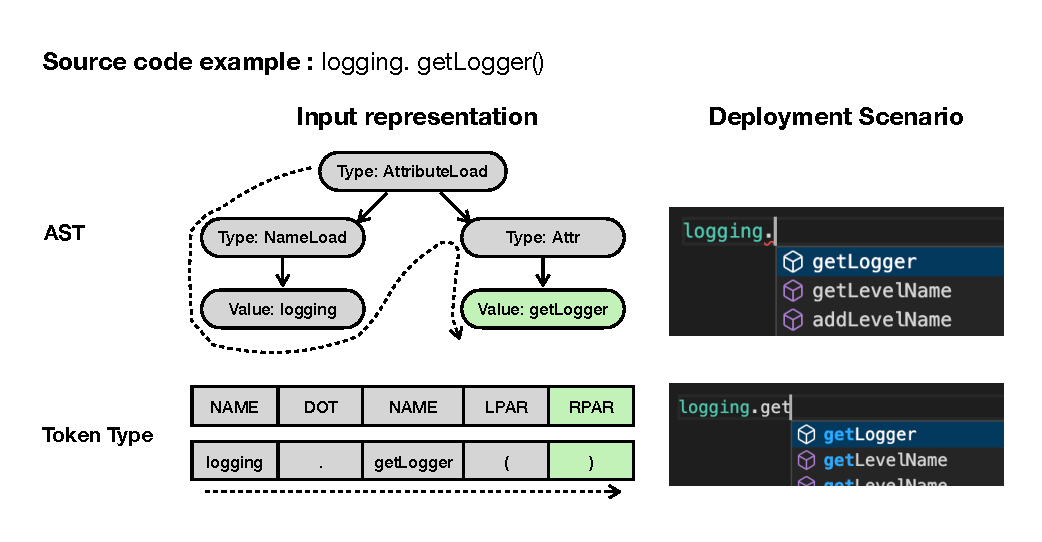
\includegraphics[width=\columnwidth]{figures/motivation.png}
%     \caption{a) source code example for parsing. b) AST parsing result c) standard token types result}
%     \label{fig:ASTfailvsType}
% \end{figure}